\documentclass[conference]{IEEEtran}
\usepackage{graphicx}
\graphicspath{{figures/}}
\usepackage{amsmath, amssymb}
\usepackage{booktabs}
\usepackage{multirow}
\usepackage{makecell}
\usepackage{array}
\usepackage[colorlinks=false,hidelinks]{hyperref}

\begin{document}

\title{MARS: A Reconfigurable Multi-Task-Capable Accelerator Architecture for Ultra-Low-Bit Streaming Inference}

\author{\IEEEauthorblockN{Po-Chun Huang\IEEEauthorrefmark{1}, Pao-Ann Hsiung\IEEEauthorrefmark{1}, and Chun-Hsian Huang\IEEEauthorrefmark{2}}
\IEEEauthorblockA{\IEEEauthorrefmark{1}Department of Computer Science and Information Engineering, National Chung Cheng University, Chiayi, Taiwan}
\IEEEauthorblockA{\IEEEauthorrefmark{2}Department of Electrical Engineering, National Chung Cheng University, Chiayi, Taiwan}}

\maketitle

\begin{abstract}
Common approaches to serving multiple AI tasks on one edge FPGA rely either on partial reconfiguration---with a fabric controller, per-task bitstreams, and millisecond-to-hundred-millisecond switches---or task sets frozen at synthesis time. We present MARS, a 1-bit-weight/1-bit-activation streaming accelerator in which one frozen backbone is shared by all tasks and a task switch is only a $\approx$25~KB parameter rewrite. Two algorithmic pieces make the ultra-low-bit adapter path work: a Residual Correction (RC) term (the adapter's pre-existing down-projection bias), with a substantially larger measured effect at 1 bit (up to $+23.0$~pp) and realised at zero additional arithmetic or datapath cost by folding it into the accumulator initial value, and multi-branch adapter scaling, which increases the effective capacity of the binary adapter path ($+3.4$~pp mean, up to $+11.3$~pp, across twenty backbone--target pairs in the deployed-geometry sweep). A 19-LUT Function Switch Controller reprograms all task-dependent parameters over one bitstream. On a PYNQ-Z2, five task-specific models switch at runtime with on-board accuracy within $0.69$~pp of software and a $1.86$~ms configuration rewrite with verified post-switch correctness; a throughput build sustains 1{,}866~img/s at 2.214~W (842.7~img/s/W) on a protocol-matched 1W1A workload with deployment-representative, different adapter geometries (Vivado-estimated FPGA power vs.\ measured GPU power).
\end{abstract}

\begin{IEEEkeywords}
FPGA accelerator, ultra-low-bit quantisation, parameter-efficient transfer learning, runtime task switching
\end{IEEEkeywords}

\section{Introduction}
Edge FPGAs increasingly serve several AI tasks from one device. The prevailing mechanism, partial reconfiguration (PR), swaps hardware regions per task and pays a fixed tax: a reconfiguration controller, a per-task partial-bitstream repository, and measured switch latencies of $5.2$~ms (ZyCAP)~\cite{Rangsikunpum2024CoarseToFine} to $97$--$114$~ms (PCAP)~\cite{Huang2024ACNNE} on PYNQ-class devices. Fixed-feature-extractor alternatives~\cite{Whatmough2019FixyNN} and on-chip variant selection~\cite{ElBouazzaoui2025NeuroAdaptive} avoid fabric rewrites but freeze the reachable task set at synthesis.

Parameter-efficient transfer learning (PEFT)~\cite{Houlsby2019Adapters,Hu2022LoRA} suggests a third path: freeze one backbone and adapt tasks through small modules such as Conv-Adapter~\cite{Chen2024ConvAdapter}. If the backbone is binarised (1W1A)~\cite{Rastegari2016XNOR,Hubara2016BinarizedNN} and mapped to a FINN-style streaming pipeline~\cite{Umuroglu2017FINN}, a task switch reduces to rewriting a small parameter set---no fabric reconfiguration at all. We find, however, that at 1 bit a single binary adapter branch exhibits a pronounced transfer-accuracy degradation, absent at comparable magnitude at ${\geq}2$ bits~\cite{Jie2023PrecisionRedundancy}.

MARS (Multi-Branch Adapter Reconfigurable Streaming-accelerator) makes the ultra-low-bit adapter path practical and verifies it on hardware. Contributions: (i) the 1-bit-specific Residual Correction finding and its zero-additional-arithmetic hardware realisation; (ii) multi-branch adapter scaling for binary networks; (iii) single-bitstream runtime task switching for eligible same-backbone tasks at $O(1)$ on-chip cost via a 19-LUT controller; and (iv) on-board verification with explicit evidence boundaries---five tasks within $0.69$~pp of software, $1.86\pm0.04$~ms configuration-rewrite switching (post-switch correctness verified), while $M{\geq}2$ branch configurations exceed the XC7Z020 and are verified at the RTL-simulation and post-synthesis levels only. To the best of our knowledge among the surveyed FPGA/PEFT accelerator works, MARS is the first to combine an ultra-low-bit shared backbone, feature-extractor-level adapters, and single-bitstream runtime task switching verified on hardware.

\section{Related Work}
\textbf{Ultra-low-bit dataflow.} BNNs replace multiply--accumulate with XNOR--popcount~\cite{Courbariaux2016BinaryConnect,Rastegari2016XNOR,Hubara2016BinarizedNN}, with representational improvements in~\cite{Liu2018BiReal,Liu2020ReActNet} and FPGA systems such as FP-BNN~\cite{Liang2018FPBNN}, and FINN-style compilers~\cite{Umuroglu2017FINN,Blott2018FINNR,Alam2023RTLMVU} and related flows~\cite{Schulte2025hls4ml} give each layer a dedicated compute unit with on-chip weights; surveys catalogue this design space~\cite{Qin2020BNNSurvey,Su2023BNNFPGASurvey,Jiang2025FPGACNNReview,Liu2024LightweightDLSurvey}---but compile one task per bitstream. \textbf{PEFT.} Adapters~\cite{Houlsby2019Adapters}, LoRA~\cite{Hu2022LoRA}, and Conv-Adapter~\cite{Chen2024ConvAdapter} adapt frozen backbones with few parameters~\cite{Belanec2025PEFTBench}, with edge-oriented CNN variants emerging~\cite{Ding2024LoRAC,Kwak2025LoRAEdge}, yet target full or moderate precision; at 1 bit the adapter itself must be binary, and its transfer effectiveness can degrade sharply~\cite{Jie2023PrecisionRedundancy}. \textbf{Task switching on FPGAs.} PR systems~\cite{Huang2024ACNNE,Rangsikunpum2024CoarseToFine} pay controller, storage, and latency costs; fixed-feature-extractor~\cite{Whatmough2019FixyNN} and variant-selection~\cite{ElBouazzaoui2025NeuroAdaptive} designs freeze the task set at synthesis. MARS occupies the unfilled point: an open set of eligible same-backbone tasks, no fabric reconfiguration, and an ultra-low-bit shared backbone.

\section{The MARS Method}
\subsection{Binary Adapter with Residual Correction}
MARS inserts one adapter beside each of the five adapter-hosting convolution layers of a frozen 1W1A VGG-like backbone (FINN's CNV: six conv + three FC layers, pre-trained on CIFAR-10). The down-projection accumulates XNOR products with 1-bit weights plus a per-channel bias,
\begin{equation}
h_j = b_j + \sum_{i=1}^{C_{\text{in}}} \operatorname{XNOR}\bigl(W^{\text{down}}_{j,i}, x_i\bigr),
\label{eq:down}
\end{equation}
followed by a binary activation $a_j = \mathbb{I}[h_j \ge 0]$ and a 1-bit up-projection $z_o = \sum_j \operatorname{XNOR}(W^{\text{up}}_{o,j}, a_j)$. The bias $b_j$ is the Residual Correction: at 1 bit, without the bias, the binary activation uses a fixed channel-wise cut that may be misaligned with the task-dependent activation distribution; RC shifts this cut. This interpretation is consistent with the observed ablation, although the complete causal pathway to final accuracy is not isolated here. In hardware, RC becomes the \emph{initial value} of the down-projection accumulator---a load the accumulator performs every window anyway---so it costs zero additional arithmetic, DSPs, or pipeline stages; only its storage and configuration bytes count, and they are included in the adapter budget. Fig.~\ref{fig:rc_hw} shows the realisation: \texttt{ram\_rc} drives the initialisation input of the accumulator multiplexer, selected at every window start.

\begin{figure}[!t]
\centering
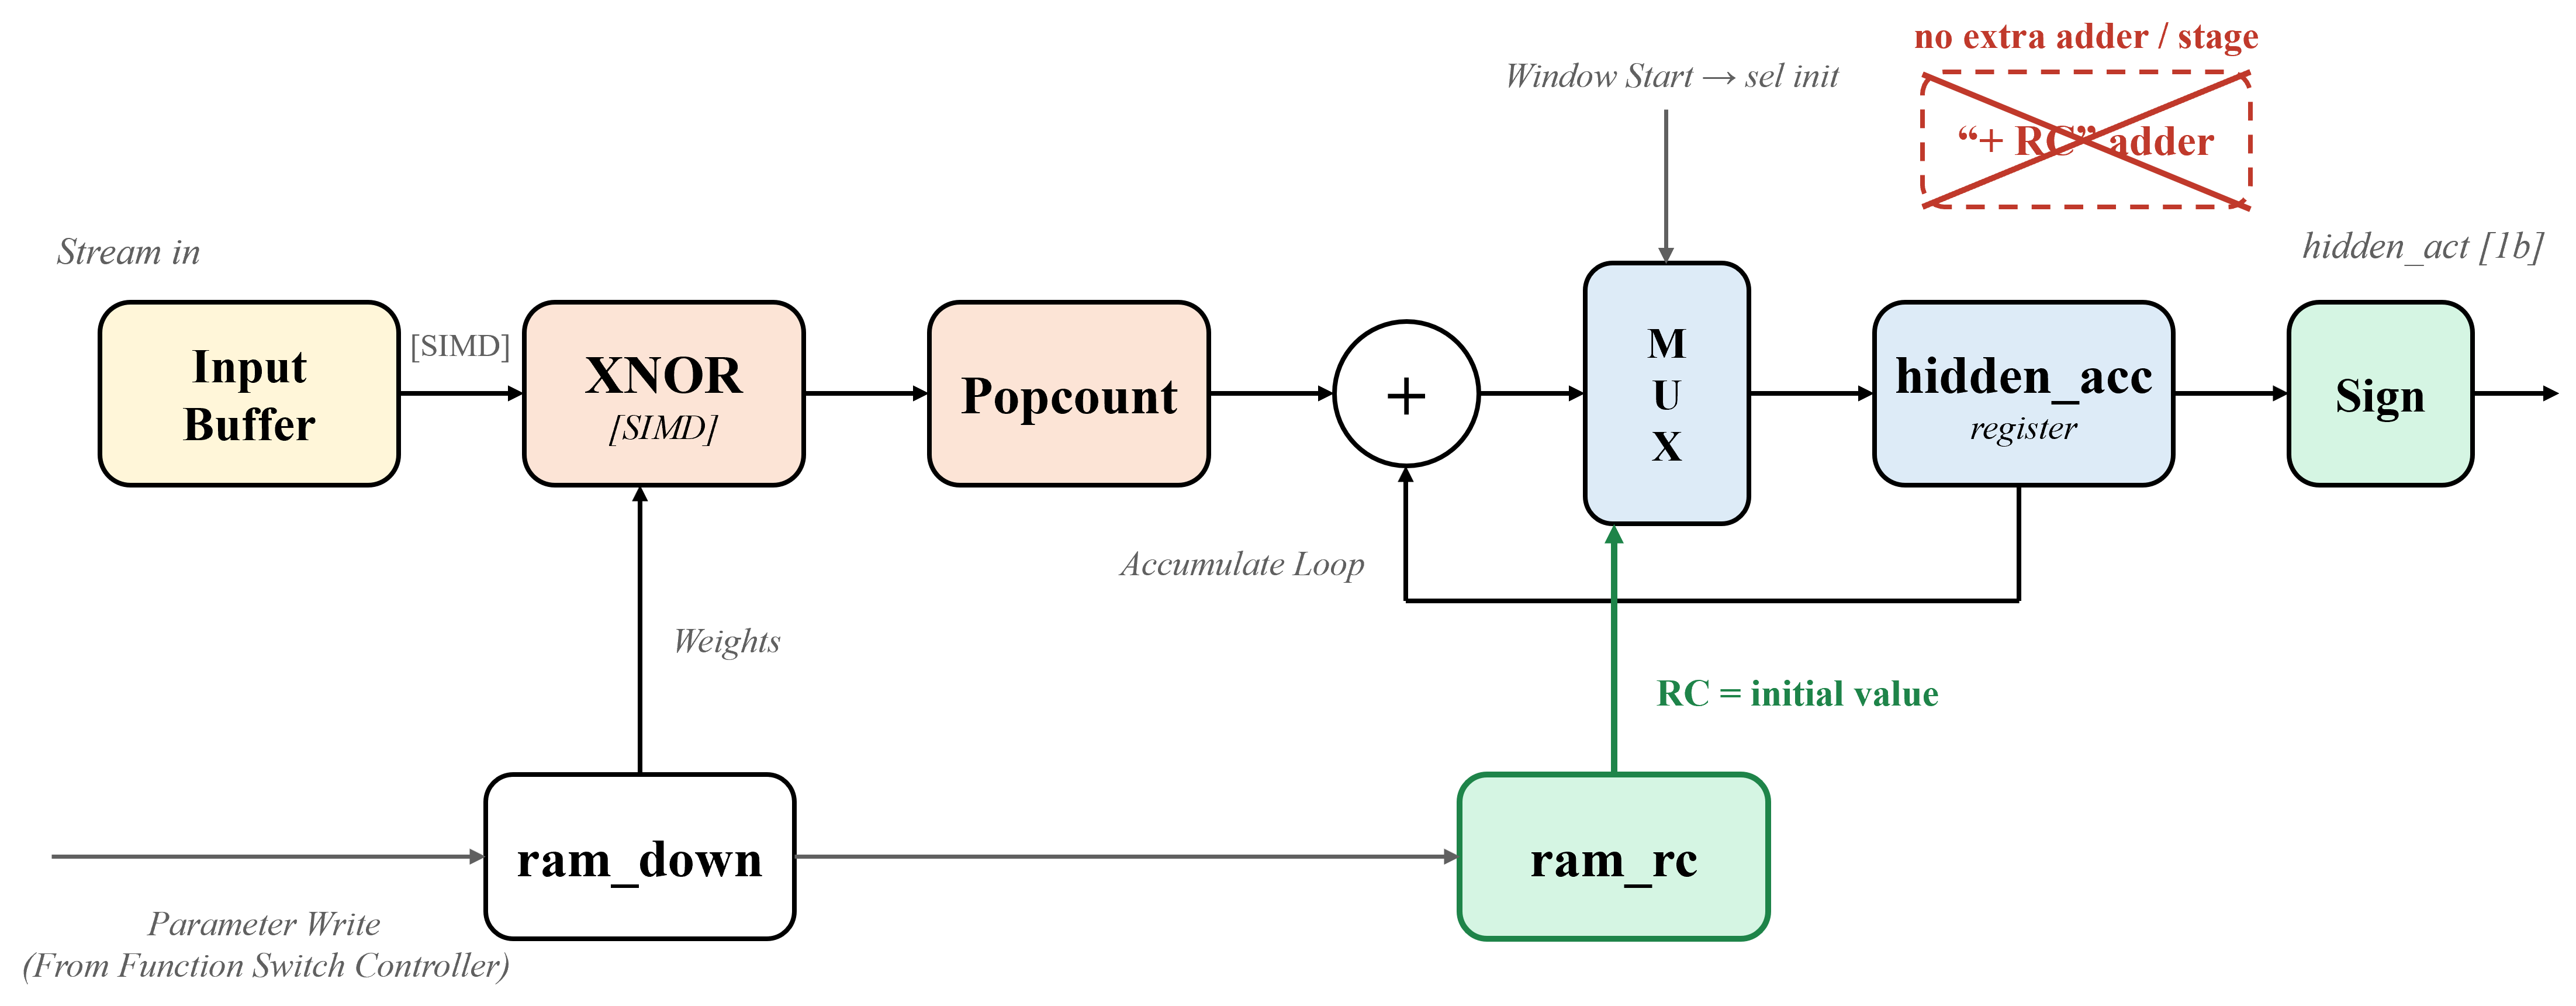
\includegraphics[width=0.84\columnwidth]{rc_in_hardware.png}
\caption{RC in hardware: accumulator initialisation from \texttt{ram\_rc}; no extra adder or pipeline stage.}
\label{fig:rc_hw}
\end{figure}

\subsection{Multi-Branch Scaling and Training}
MARS sums $M$ structurally identical branches with independent weights, RC, and scales,
\begin{equation}
y_o = \sum_{i=1}^{M} \alpha_i\, z_o^{(i)},
\label{eq:mb}
\end{equation}
enriching the integer-valued corrections the adapter can express (each branch output is itself multi-level; no fixed level count is claimed). The overhead is linear: $+58{,}533$ parameters ($+3.78\%$ of the backbone) and $+4.23$~MMACs per branch (compute-then-crop software reference; the deployed RTL's centre-selection evaluates $3.01$~MMACs). Training freezes the backbone and updates the adapter and classifier jointly: weights binarise in the forward pass ($W = \operatorname{sign}(\widetilde{W})$) with the straight-through estimator $\partial \operatorname{sign}(u)/\partial u \approx \mathbf{1}_{|u|\le 1}$ in the backward pass, while each real-valued scale receives the exact gradient $\partial L/\partial \alpha_i = \langle \partial L/\partial y, z^{(i)} \rangle$. At export, $\alpha_i$ is quantised into a Q8 contribution look-up table and RC into the accumulator initial value.

\section{Hardware Architecture}
\subsection{Streaming Pipeline and Super Wrapper}
Fig.~\ref{fig:arch} shows the deployed system on a Zynq XC7Z020 at 100~MHz: MVAU0, five adapter-enhanced Super Wrappers (Super1--5), and MVAU6--8, with a Function Switch Controller (FSC) fanning a configuration bus out to all task-dependent memories. In a FINN pipeline, thresholding happens inside each matrix--vector--activation unit, so raw partial sums are not normally exposed; the Super Wrapper (Fig.~\ref{fig:wrapper}) decouples that thresholding, duplicates the input stream to the modified MVAU core and the Adapter IP, synchronises the adapter side-stream through a small FIFO, and fuses both before one shared Q8 threshold:
\begin{equation}
\hat{y}_o = \mathbb{I}\bigl[(p_o \ll 8) + s_o \cdot \mathrm{LUT}_{\alpha}(q_o) \ge T^{Q8}_o\bigr],
\label{eq:fusion}
\end{equation}
with $p_o$ the backbone partial sum, $q_o$ the up-projection popcount, and $T^{Q8}_o$ the BatchNorm-fused threshold---shifts, look-ups, and integer adds only. All adapter memories are configuration-writable distributed RAM, so the adapter adds zero BRAM and zero DSPs.

\begin{figure}[!t]
\centering
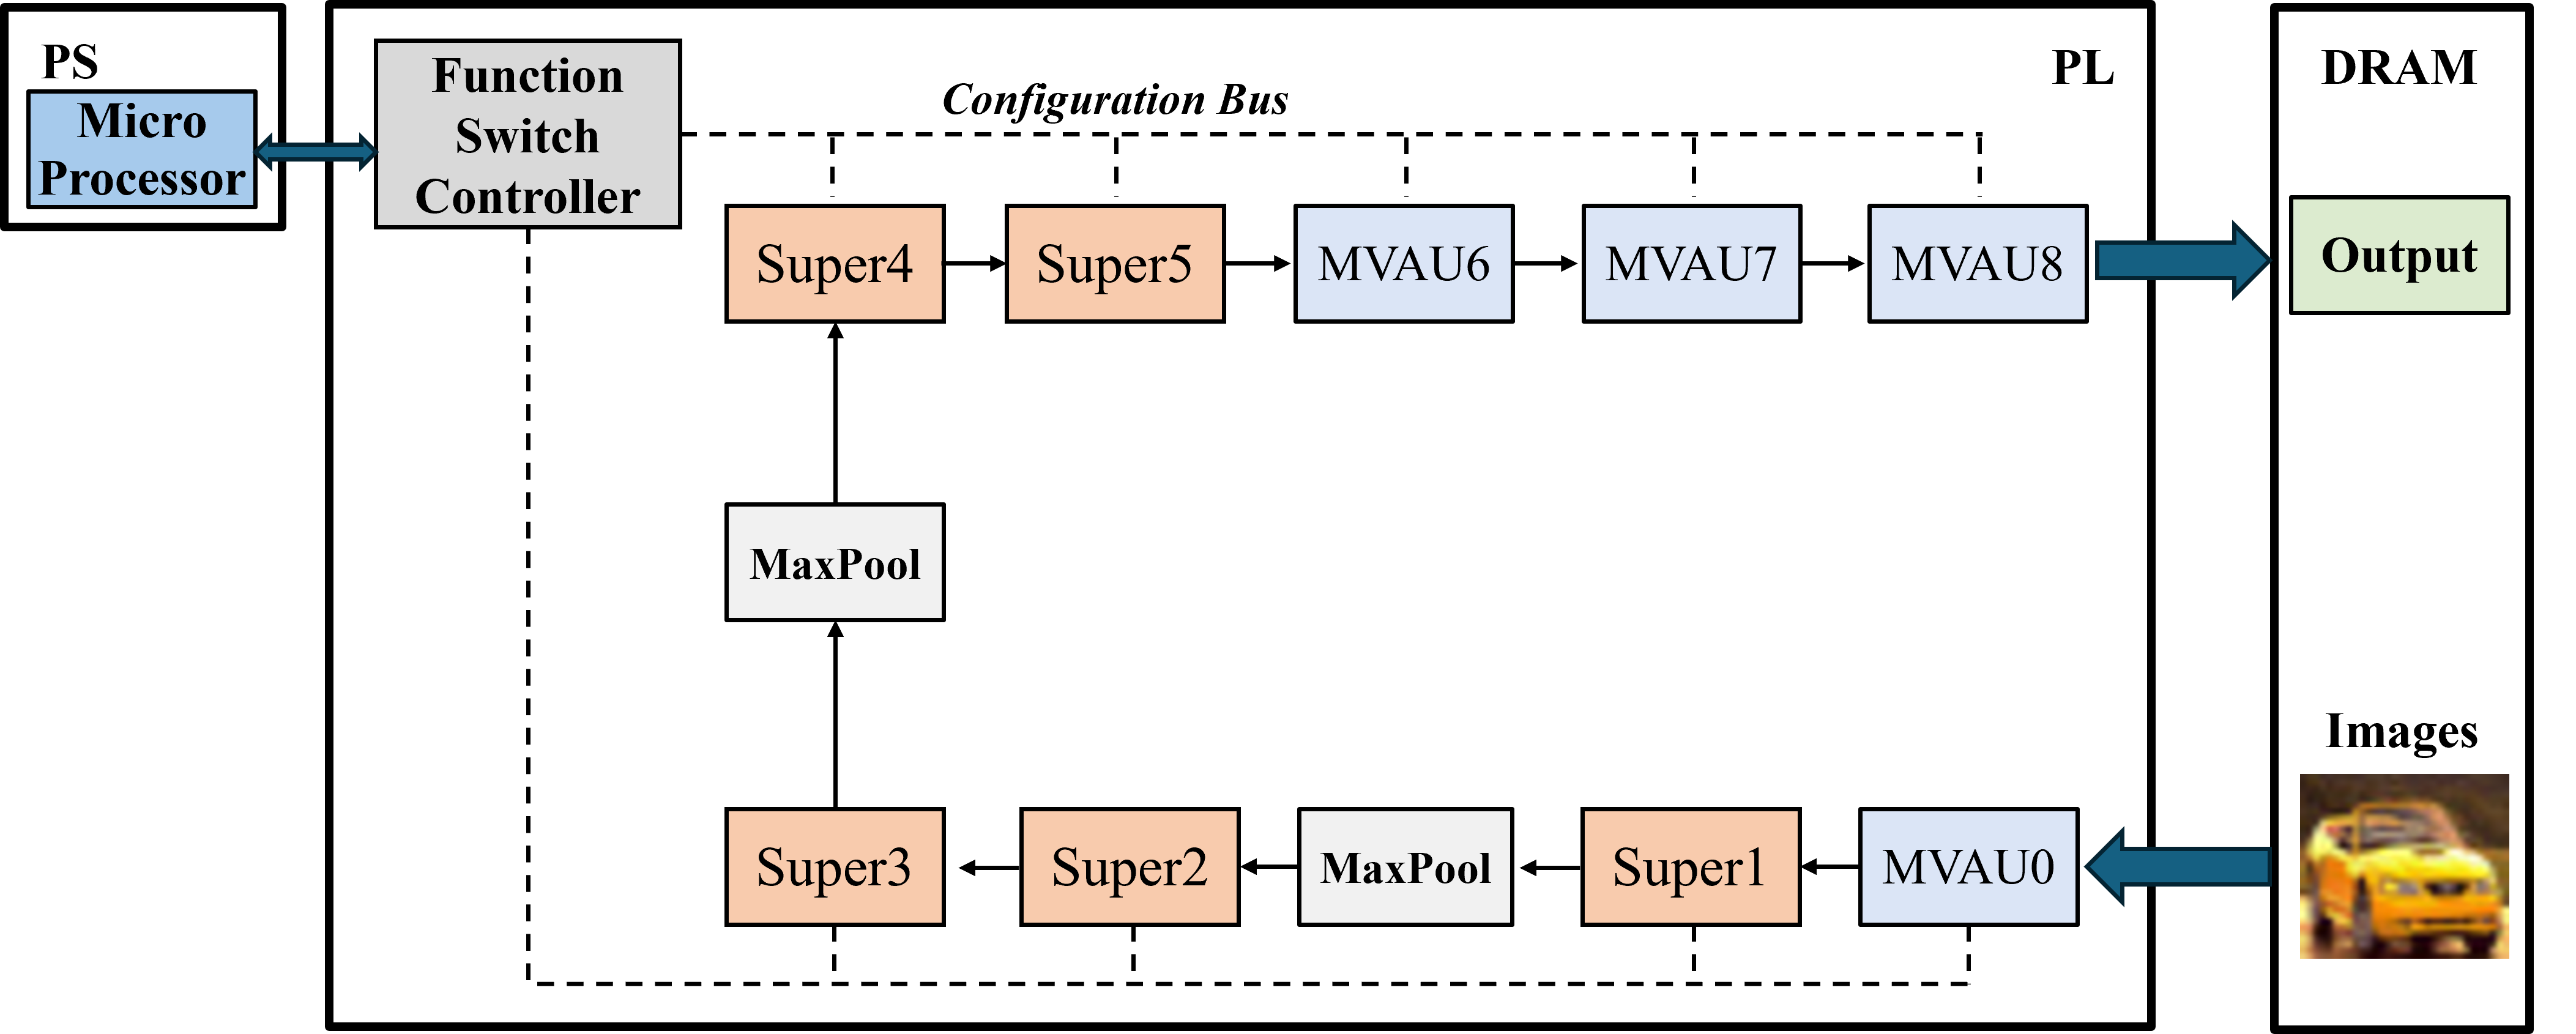
\includegraphics[width=\columnwidth]{fig44_mars_arch.png}
\caption{MARS streaming dataflow: MVAU0, adapter-enhanced Super1--5, MVAU6--8, and the Function Switch Controller.}
\label{fig:arch}
\end{figure}

\begin{figure}[!t]
\centering
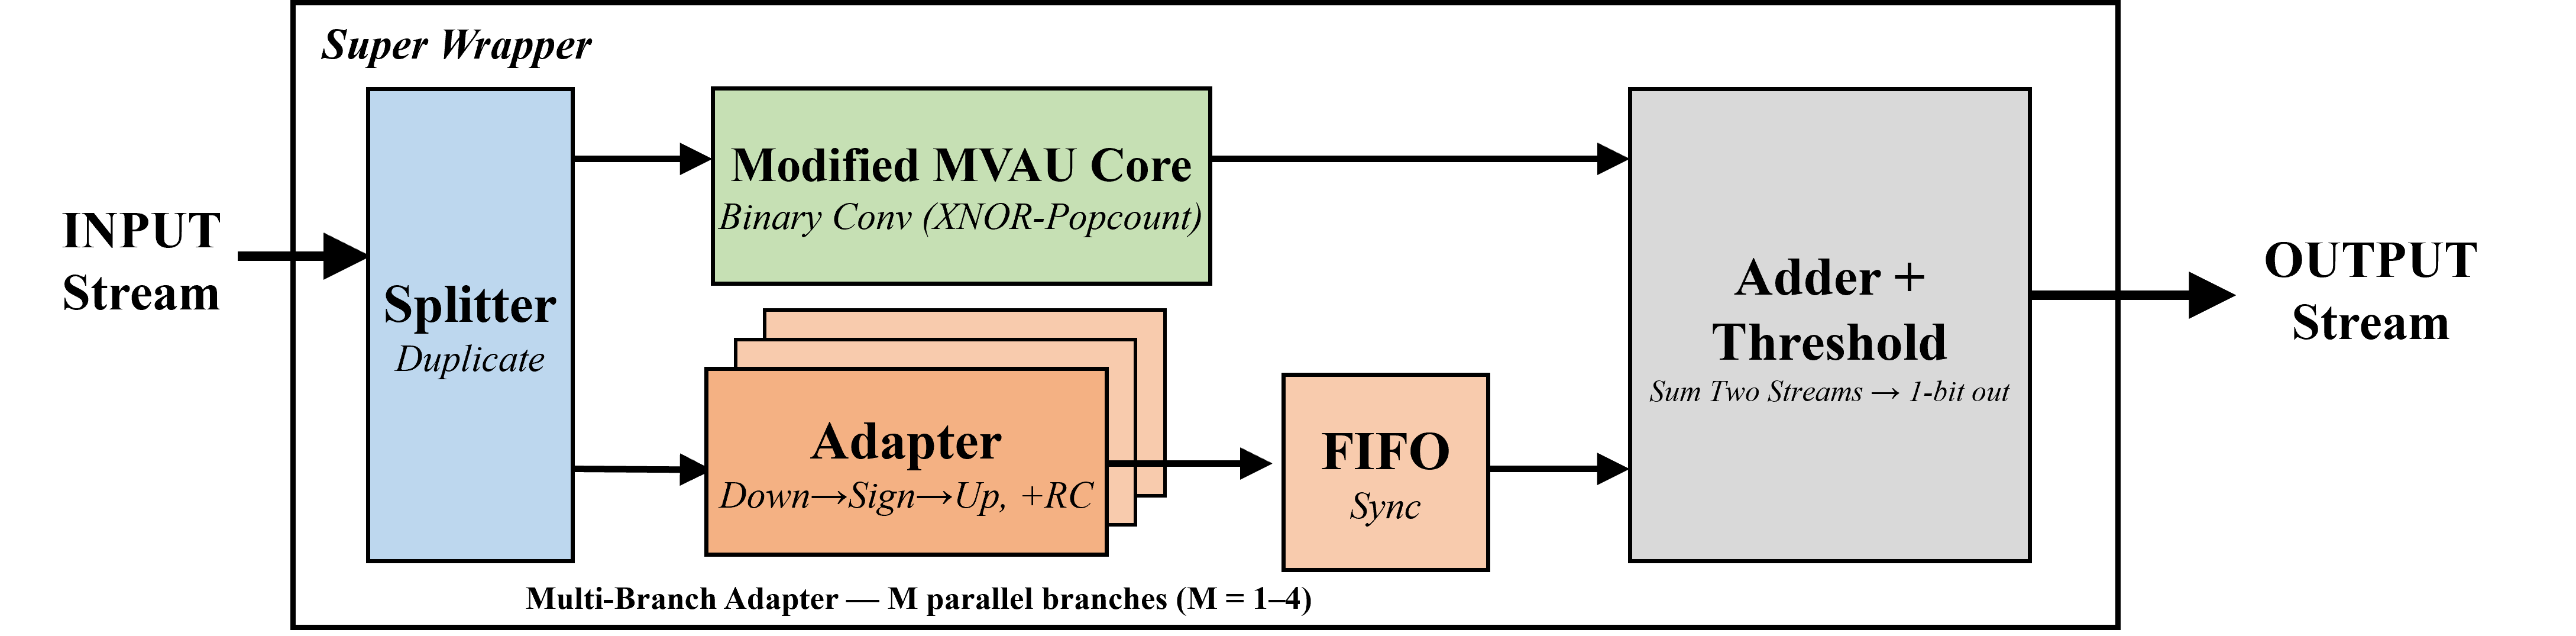
\includegraphics[width=\columnwidth]{hw_super_wrapper.png}
\caption{Super Wrapper: the modified MVAU core exposes raw partial sums; the adapter contribution is fused before the shared Q8 threshold.}
\label{fig:wrapper}
\end{figure}

\subsection{Runtime Task Switching}
The FSC is a 19-LUT AXI-Lite slave that decodes a 64~KB aperture into nine destinations (MVAU0 thresholds, MVAU8 classifier weights, five adapter blobs, MVAU6/7 thresholds). Because all eligible tasks share the frozen backbone, only BatchNorm-fused thresholds, the classifier projection, and adapter parameters differ per task: a full switch is a $\approx$25~KB rewrite (25{,}088 stored B; 6{,}757 32-bit writes = 27{,}028 bus B, sub-word fields widened on the bus)---wait for the output-DMA done flag, bulk-write the blob, launch the next batch; no additional flush beyond the output-DMA-done barrier, no fabric reconfiguration (Fig.~\ref{fig:switch}). Each additional task is an off-line host-side blob: on-chip cost is $O(1)$ in the task count for same-backbone, $32{\times}32{\times}3$, same-output-head classification tasks. Two builds realise two depths of this mechanism: a \emph{throughput} build (FINN-default folding, one adapter task baked at synthesis, 2-task) and a \emph{compactness} build (uniform PE${=}1$, memories power up empty, any eligible same-backbone task loadable at runtime, $N$-task).

\begin{figure}[!t]
\centering
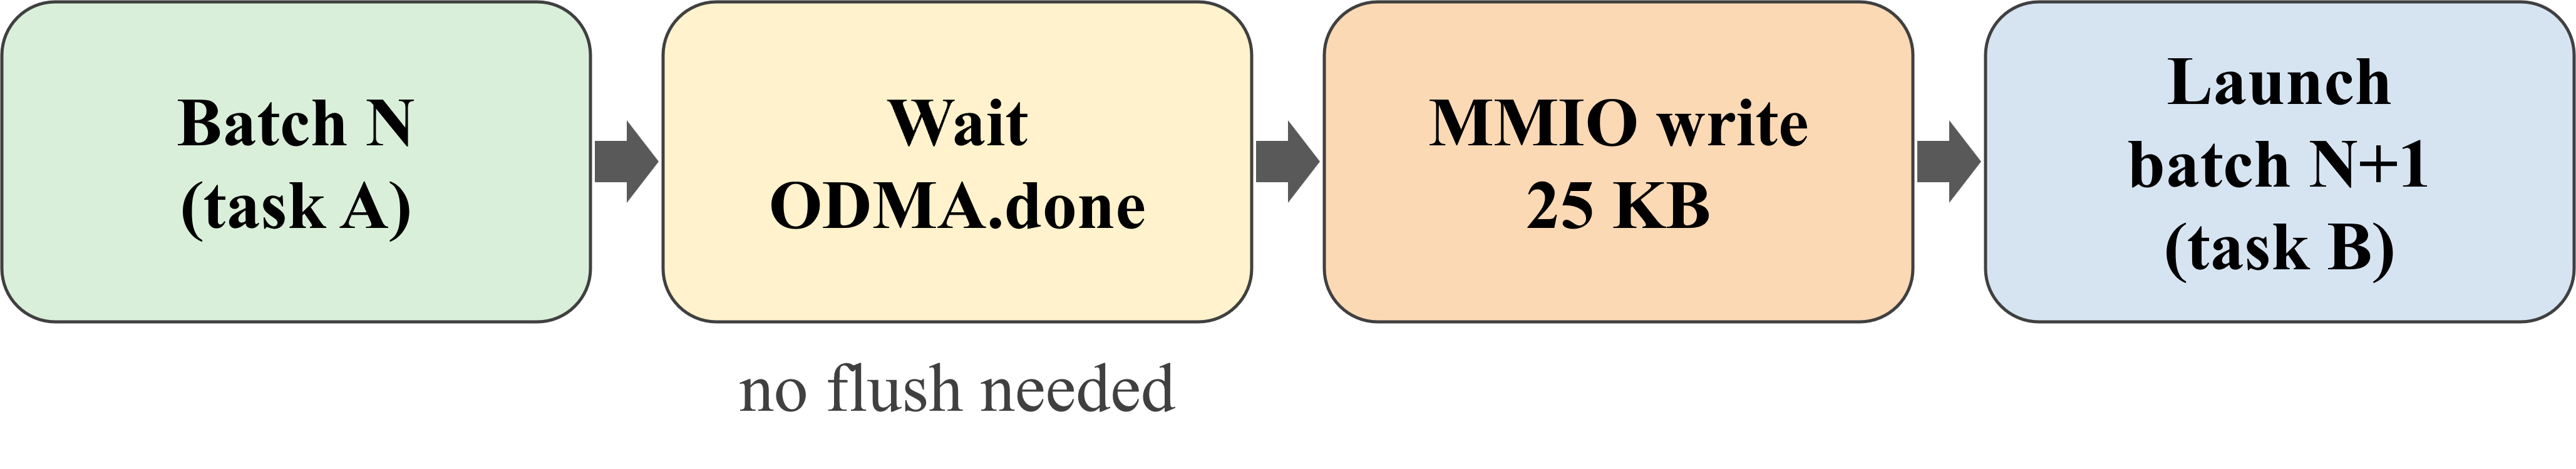
\includegraphics[width=0.86\columnwidth]{task_switch.png}
\caption{Runtime task-switching sequence.}
\label{fig:switch}
\end{figure}

\section{Experimental Results}
\textbf{Setup.} PyTorch + Brevitas~\cite{Pappalardo2021Brevitas} QAT (200 epochs, ADAM, lr 0.005, seed 2024); FINN + Vivado 2022.2; PYNQ-Z2 (XC7Z020). Five $32{\times}32{\times}3$ datasets: CIFAR-10 (backbone), SVHN, FashionMNIST, STL10, CINIC10. Correctness is verified at three levels: per-module RTL simulation (43{,}520 vectors, 100\% bit-exact), top-level dataflow simulation against the PyTorch golden model, and on-board execution. Accuracies are best-epoch operating points selected on the test split (original BNN-PYNQ trainer flow; the identical rule for every configuration).

\textbf{RC at 1 bit.} Table~\ref{tab:rc} isolates RC on CIFAR-10$\to$SVHN: $+15$ to $+17$~pp at every branch count in the wide geometry and $+23.0$~pp in the deployed geometry, while at ${\geq}2$ bits the same term is typically within $\pm 0.3$~pp (maximum observed $1.4$~pp). Gains on other targets range from $+0.6$ to $+7.4$~pp.

\begin{table}[!t]
\centering
\caption{RC ablation at 1 bit, wide geometry (CIFAR-10 $\to$ SVHN).}
\label{tab:rc}
\small
\setlength{\tabcolsep}{4pt}
\resizebox{\columnwidth}{!}{%
\begin{tabular}{llrrrr}
\toprule
\textbf{Adapter} & \textbf{M} & \textbf{No-RC} & \textbf{With RC} & \textbf{$\Delta_{\text{RC}}$} & \textbf{Full-FT} \\
\midrule
Conv-Adapter~\cite{Chen2024ConvAdapter} & 1 & 63.06\% & 79.23\% & +16.17 & \multirow{4}{*}{94.91\%} \\
\cmidrule(lr){1-5}
\multirow{3}{*}{\textbf{MARS}} & 2 & 66.12\% & 83.01\% & +16.89 & \\
 & 3 & 67.79\% & 83.48\% & +15.69 & \\
 & 4 & 69.08\% & \textbf{84.44\%} & +15.36 & \\
\bottomrule
\end{tabular}%
}
\end{table}

\textbf{Multi-branch scaling.} Across twenty backbone--target pairs spanning five source backbones, the deployed-geometry sweep (Table~\ref{tab:mbdep}) raises 1-bit transfer accuracy by $+3.36$~pp on average over the single-branch baseline, up to $+11.33$~pp (FashionMNIST$\to$SVHN), with the largest gains on hard transfers and diminishing returns as $M$ grows. Table~\ref{tab:mbsw} shows the complementary wide-geometry software study on the CIFAR-10 backbone. Every one of the twenty pairs improves (largest: FashionMNIST$\to$SVHN $+11.33$~pp, STL10$\to$SVHN $+7.50$~pp, CINIC10$\to$SVHN $+7.20$~pp); five paired seeds provide preliminary evidence of a positive $M{=}1{\to}4$ gain on two deployment-relevant transfers under the same test-selected checkpoint protocol: $+6.64\pm0.43$~pp on SVHN and $+2.69\pm0.36$~pp on FashionMNIST; a selection-free final-epoch reading of the same logs yields consistent gains ($+6.87$/$+2.99$~pp).

\begin{table}[!t]
\centering
\caption{Deployed-geometry multi-branch transfer accuracy (\%) over all twenty backbone--target pairs ($M{=}1$ vs.\ $M{=}4$, RC on; single seed). $\Delta_{\text{multi}} = M{=}4 - M{=}1$ (pp).}
\label{tab:mbdep}
\small
\setlength{\tabcolsep}{5pt}
\begin{tabular}{llccc}
\toprule
\textbf{Backbone} & \textbf{Target} & $M{=}1$ & $M{=}4$ & $\Delta_{\text{multi}}$ \\
\midrule
CIFAR-10 & SVHN & 73.72 & 79.81 & $+6.09$ \\
 & FashionMNIST & 80.42 & 83.54 & $+3.12$ \\
 & STL10 & 67.46 & 68.06 & $+0.60$ \\
 & CINIC10 & 64.80 & 65.45 & $+0.65$ \\
SVHN & CIFAR-10 & 43.18 & 48.37 & $+5.19$ \\
 & FashionMNIST & 78.51 & 81.89 & $+3.38$ \\
 & STL10 & 34.41 & 35.10 & $+0.69$ \\
 & CINIC10 & 33.59 & 38.03 & $+4.44$ \\
STL10 & CIFAR-10 & 66.65 & 68.79 & $+2.14$ \\
 & FashionMNIST & 81.48 & 84.19 & $+2.71$ \\
 & SVHN & 68.15 & 75.65 & $+7.50$ \\
 & CINIC10 & 54.26 & 56.56 & $+2.30$ \\
FashionMNIST & CIFAR-10 & 33.63 & 36.76 & $+3.13$ \\
 & STL10 & 32.64 & 34.11 & $+1.47$ \\
 & SVHN & 51.37 & 62.70 & $+11.33$ \\
 & CINIC10 & 27.75 & 29.56 & $+1.81$ \\
CINIC10 & CIFAR-10 & 78.21 & 78.72 & $+0.51$ \\
 & SVHN & 69.14 & 76.34 & $+7.20$ \\
 & STL10 & 67.21 & 67.42 & $+0.21$ \\
 & FashionMNIST & 80.23 & 82.88 & $+2.65$ \\
\midrule
\multicolumn{2}{l}{Mean gain over $M{=}1$ (pp)} & --- & --- & $+3.36$ \\
\bottomrule
\end{tabular}
\end{table}

\begin{table}[!t]
\centering
\caption{Multi-branch scaling on the CIFAR-10 backbone (wide geometry, software, 1W1A, RC).}
\label{tab:mbsw}
\small
\setlength{\tabcolsep}{3.5pt}
\resizebox{\columnwidth}{!}{%
\begin{tabular}{lccccc}
\toprule
 & \textbf{\cite{Chen2024ConvAdapter}} & \multicolumn{3}{c}{\textbf{MARS}} & \\
\cmidrule(lr){2-2}\cmidrule(lr){3-5}
\textbf{Target} & \textbf{$M{=}1$} & \textbf{$M{=}2$} & \textbf{$M{=}3$} & \textbf{$M{=}4$} & \textbf{Full-FT} \\
\midrule
SVHN         & 79.23 & 83.01 & 83.48 & \textbf{84.44} & 94.91 \\
STL10        & 67.50 & 67.48 & 67.68 & \textbf{68.15} & 71.05 \\
FashionMNIST & 82.71 & 83.57 & \textbf{83.63} & 83.60 & 92.36 \\
CINIC10      & 64.50 & 64.71 & 64.85 & \textbf{65.02} & 68.02 \\
\bottomrule
\end{tabular}%
}
\end{table}

\begin{figure}[!t]
\centering
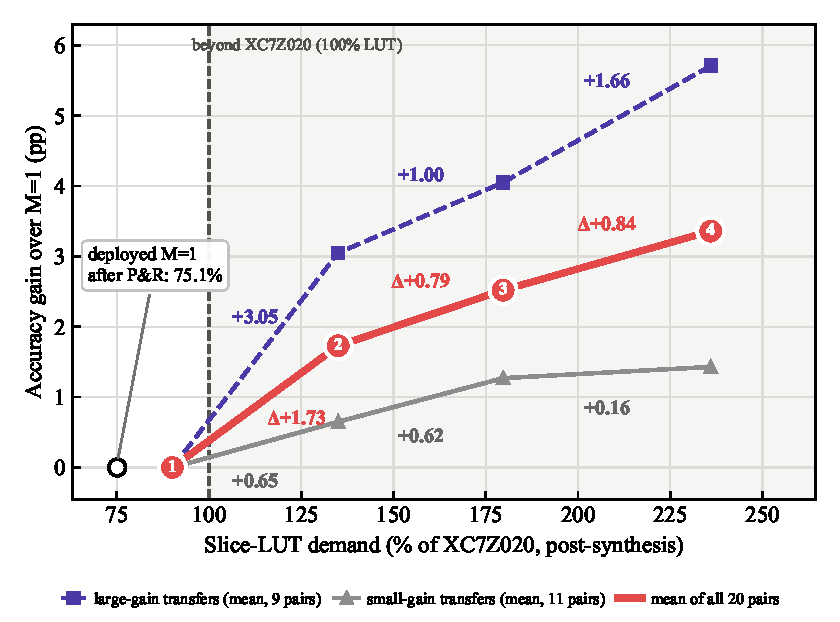
\includegraphics[width=0.9\columnwidth]{mb_tradeoff_compact_lut.pdf}
\caption{Accuracy gain vs.\ post-synthesis LUT demand for branch scaling (compactness build; large-gain: $\Delta_{\text{multi}} \geq 3$~pp, 9 pairs vs.\ 11); $M{\geq}2$ exceeds the XC7Z020.}
\label{fig:tradeoff}
\end{figure}

\textbf{On-board task switching.} Table~\ref{tab:onboard}: the five task-specific models served from the single compactness bitstream (loaded in turn from host-resident images) each reproduce their software reference within $0.69$~pp (10{,}000-image test sets; STL10 its full 8{,}000); the residual gap is consistent with fixed-point and threshold-quantisation effects; no mismatch was observed in the per-module RTL tests. Fifty random switches give a $1.86\pm0.04$~ms configuration rewrite (post-switch correctness verified separately), $\approx$0.02\% of a batch-1000 run. Compared with published task-switching FPGA inference (Table~\ref{tab:prior}), MARS is the only surveyed system needing no fabric-PR controller while keeping the task set open after synthesis.

\begin{table}[!t]
\centering
\caption{On-board $N$-task switching accuracy (compactness build).}
\label{tab:onboard}
\small
\resizebox{\columnwidth}{!}{%
\begin{tabular}{llrrr}
\toprule
\textbf{Dataset} & \textbf{Mode} & \textbf{Software Reference} & \textbf{On-Board} & \textbf{Gap (pp)} \\
\midrule
CIFAR-10     & backbone only & 81.46\% & 80.99\% & $-0.47$ \\
SVHN         & MARS          & 73.72\% & 73.21\% & $-0.51$ \\
FashionMNIST & MARS          & 80.42\% & 79.98\% & $-0.44$ \\
STL10        & MARS          & 67.46\% & 66.77\% & $-0.69$ \\
CINIC10      & MARS          & 64.80\% & 64.64\% & $-0.16$ \\
\bottomrule
\end{tabular}%
}
\end{table}

\begin{table}[!t]
\centering
\caption{Task-switching FPGA inference vs.\ published approaches. Latencies correspond to different switching semantics; the adaptation level and residency model differ across approaches.}
\label{tab:prior}
\small
\setlength{\tabcolsep}{3pt}
\resizebox{\columnwidth}{!}{%
\begin{tabular}{lrcl}
\toprule
\textbf{Approach} & \makecell{\textbf{Switch}\\\textbf{Latency}} & \makecell{\textbf{PR}\\\textbf{Ctrl.}} & \textbf{Task Storage Scaling} \\
\midrule
ACNNE~\cite{Huang2024ACNNE}          & 97--114~ms & Yes & partial bitstream / task \\
CoarseToFine~\cite{Rangsikunpum2024CoarseToFine} & 5.2~ms & Yes & partial bitstream / task \\
FixyNN~\cite{Whatmough2019FixyNN}    & N/A        & No  & back-end HW / task \\
NeuroAdaptive~\cite{ElBouazzaoui2025NeuroAdaptive} & 0.23--0.67~$\mu$s & No & on-chip, fixed at synthesis \\
\midrule
\textbf{MARS} & \textbf{1.86~ms} & \textbf{No} & \textbf{$O(1)$ on-chip; 25~KB blob / task} \\
\bottomrule
\end{tabular}%
}
\end{table}

Table~\ref{tab:cost} itemises the per-branch cost, and Table~\ref{tab:twovsn} contrasts how the two builds realise two depths of the same switching mechanism.

\begin{table}[!t]
\centering
\caption{Per-branch parameter and post-synthesis cost (compactness).}
\label{tab:cost}
\small
\setlength{\tabcolsep}{3.5pt}
\resizebox{\columnwidth}{!}{%
\begin{tabular}{ccccc}
\toprule
\textbf{M} & \textbf{Params} & \textbf{vs.\ Backbone} & \textbf{Slice LUTs (\%)} & \textbf{Power (W)} \\
\midrule
1 & 58{,}533  & $+3.78\%$  & 47{,}931 (90.1\%)   & 1.841 \\
2 & 117{,}066 & $+7.57\%$  & 71{,}841 (135.0\%)  & 1.897 \\
3 & 175{,}599 & $+11.35\%$ & 95{,}593 (179.7\%)  & 1.915 \\
4 & 234{,}132 & $+15.14\%$ & 125{,}538 (236.0\%) & 1.969 \\
\bottomrule
\end{tabular}%
}
\end{table}

\begin{table}[!t]
\centering
\caption{Two-task vs.\ $N$-task switching.}
\label{tab:twovsn}
\small
\setlength{\tabcolsep}{3pt}
\resizebox{\columnwidth}{!}{%
\begin{tabular}{lll}
\toprule
 & \textbf{Throughput (2-task)} & \textbf{Compactness ($N$-task)} \\
\midrule
Folding & heterog.\ PE $\le 32$ & uniform PE = 1 \\
Baked at synthesis & one adapter task & nothing \\
Moved per switch & $\approx$15 KB & full blob $\approx$25 KB \\
Reachable models & exactly two & any eligible same-backbone task \\
Verified & on-board, 2 tasks & on-board, 5 tasks \\
\bottomrule
\end{tabular}%
}
\end{table}

\begin{figure}[!t]
\centering
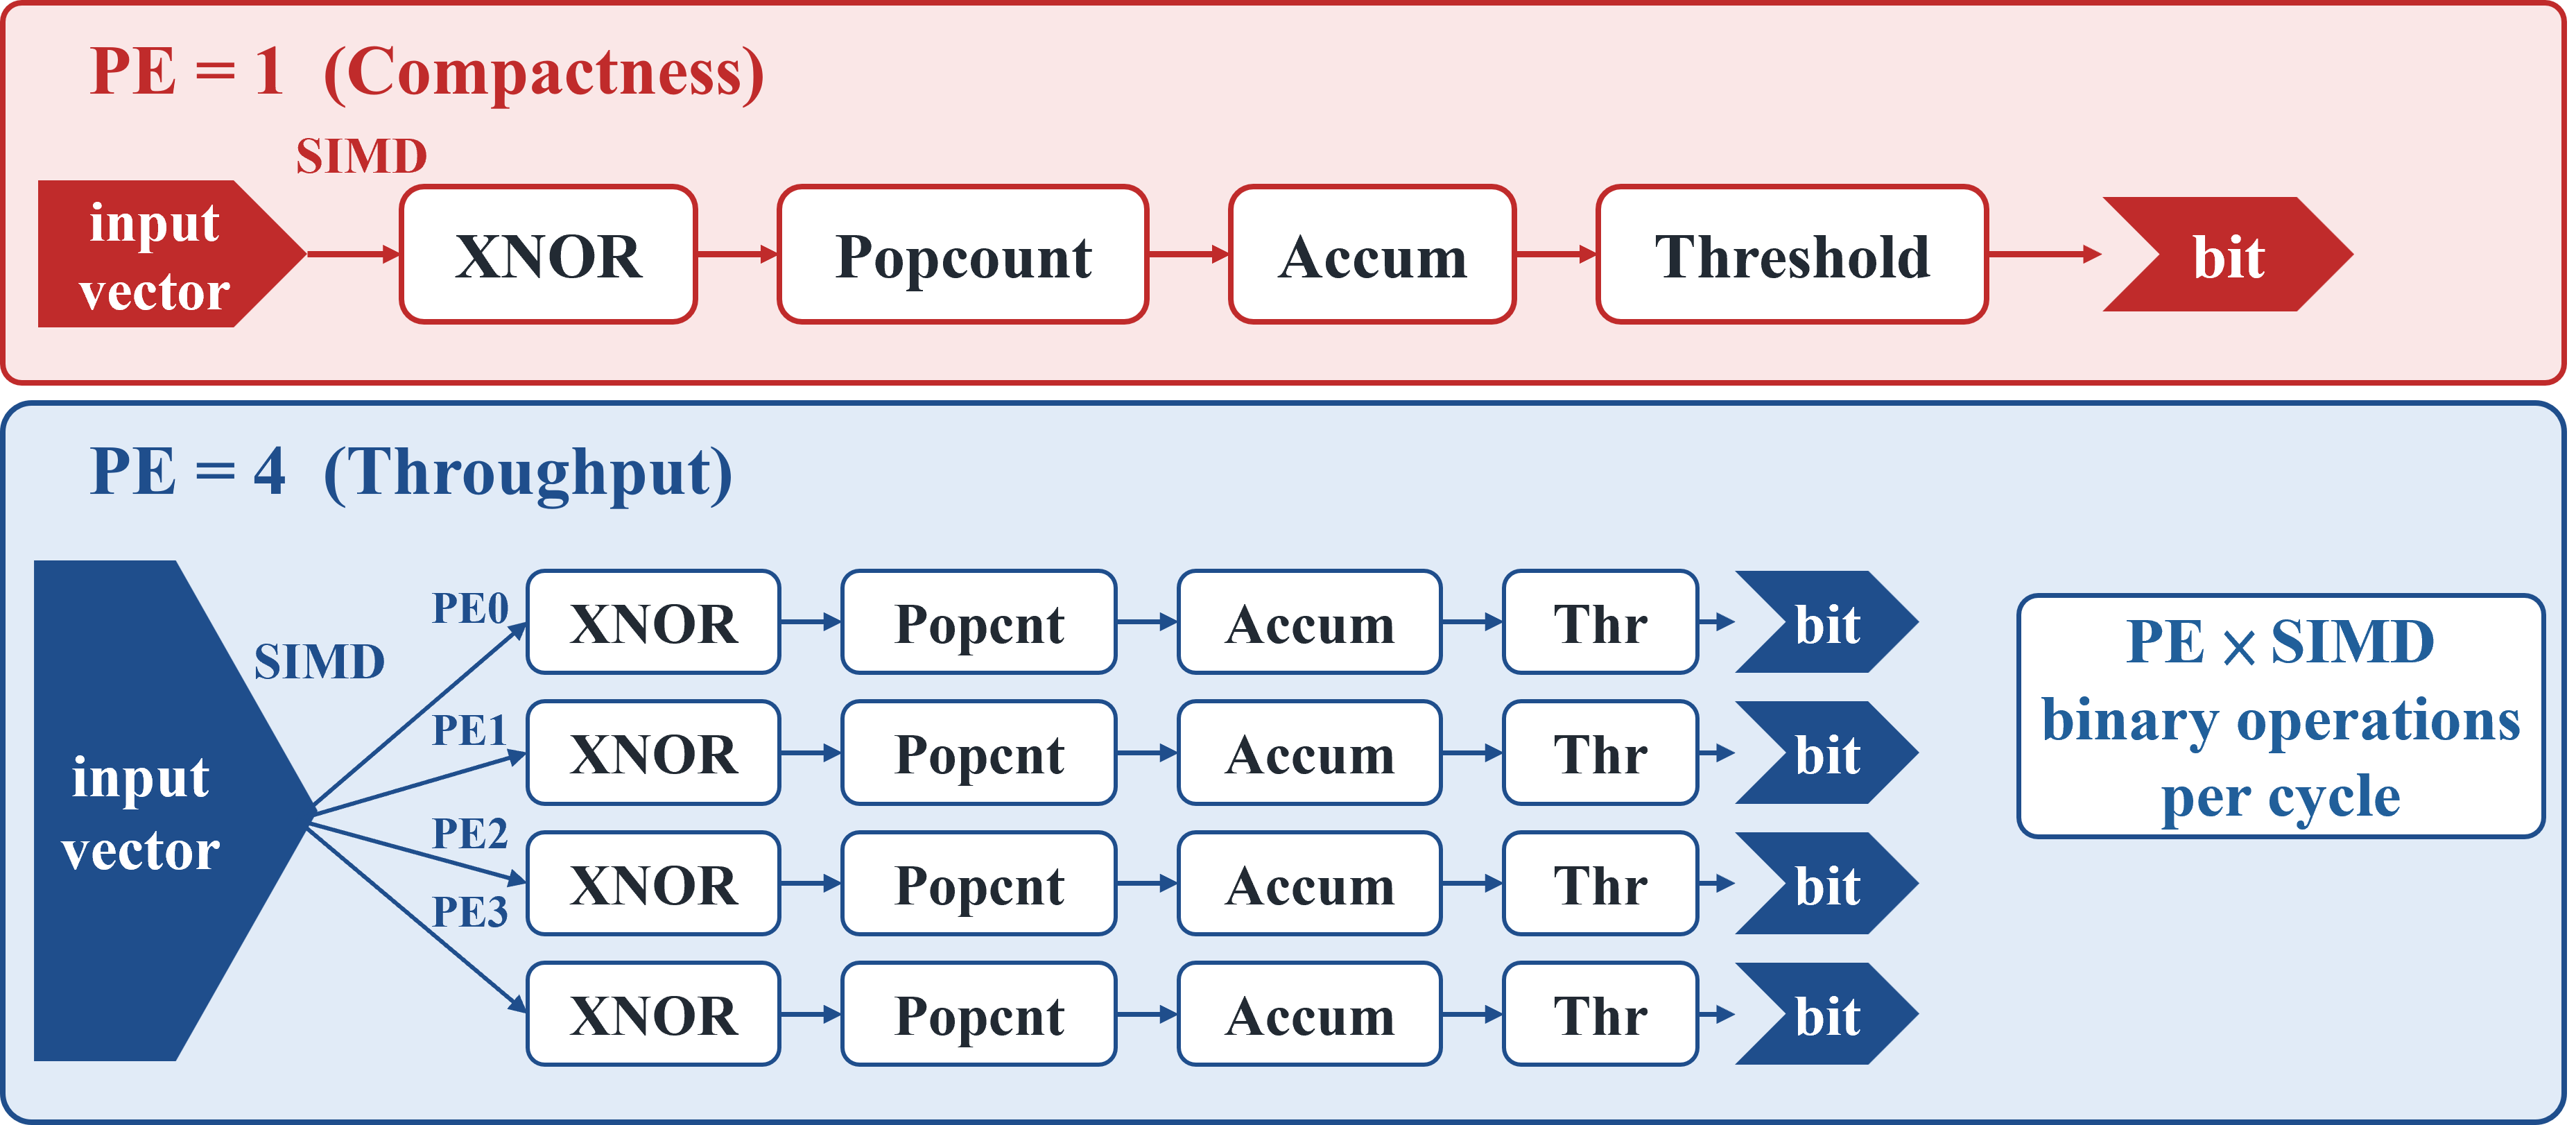
\includegraphics[width=0.84\columnwidth]{pe_diff.png}
\caption{Folding difference between the builds: PE${=}1$ (compactness) vs.\ PE-parallel lanes (throughput, illustrated for PE${=}4$).}
\label{fig:pe_diff}
\end{figure}

Fig.~\ref{fig:layout} shows the post-implementation placement of the compactness build: adapter logic and backbone MVAUs dominate and interleave across the die, while the FSC appears only as a negligible scattering of cells, matching its 19-LUT footprint. The $1.86$~ms switch amortises to $\approx$0.02\% of a batch-1000 run; serving $T$ tasks requires one bitstream plus $T$ host-side 25~KB blobs, versus $T$ partial bitstreams for PR systems.

\begin{figure}[!t]
\centering
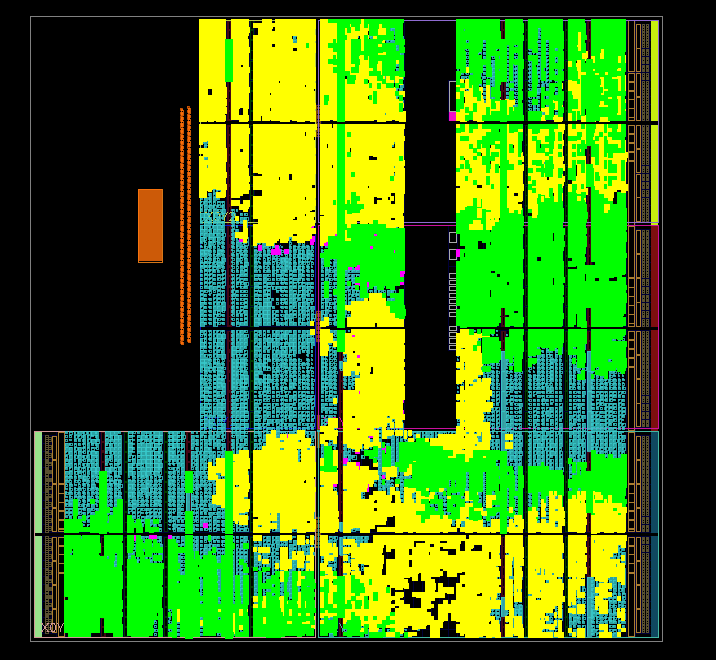
\includegraphics[width=0.72\columnwidth]{mars_soc_layout.png}
\caption{Layout of the compactness build (XC7Z020). Yellow: adapter + adapter RAM; green: MVAUs; purple: FSC; orange: PS; blue: other SoC logic.}
\label{fig:layout}
\end{figure}

\textbf{Cross-platform.} On a protocol-matched 1W1A SVHN workload at batch 1000 (Table~\ref{tab:xplat}), the throughput build sustains 1{,}866~img/s at 2.214~W---842.7~img/s/W, $11.9\times$ the RTX~4090 and $5.9\times$ the Jetson Orin~NX. FPGA power is the Vivado post-route estimate while GPU/Jetson power is runtime-measured (NVML/tegrastats), so the ratios are specific to this workload and measurement methodology, not a general platform-efficiency claim; the GPU/Jetson run the $3{\times}3$ Conv-Adapter geometry while the FPGA runs the deployed $1{\times}1$ MARS geometry (a deployment-level comparison, not a same-model sweep).

\begin{table}[!t]
\centering
\caption{Deployment-level comparison, matched protocol but different adapter geometries (SVHN, batch 1000).}
\label{tab:xplat}
\small
\setlength{\tabcolsep}{3pt}
\resizebox{\columnwidth}{!}{%
\begin{tabular}{lrrrr}
\toprule
\textbf{Metric} & \makecell{\textbf{RTX}\\\textbf{4090}} & \makecell{\textbf{Orin}\\\textbf{NX}} & \makecell{\textbf{MARS}\\\textbf{(Compact.)}} & \makecell{\textbf{MARS}\\\textbf{(Thrput.)}} \\
\midrule
Adapter geometry     & $3{\times}3$ wide & $3{\times}3$ wide & $1{\times}1$ depl. & $1{\times}1$ depl. \\
FPS (img/s)          & 9{,}388 & 2{,}752 & 107.1 & 1{,}866 \\
Power (W)            & 132.48  & 19.23   & 1.802 & 2.214 \\
Efficiency (img/s/W) & 70.86   & 143.1   & 59.4  & \textbf{842.7} \\
\bottomrule
\end{tabular}%
}
\end{table}

\section{Discussion and Limitations}
The two builds are complementary operating points: the throughput build for a fixed task (or task pair) known at synthesis, the compactness build when the task set must stay open---its throughput cost is the PE${=}1$ folding (Fig.~\ref{fig:pe_diff}), not the switching machinery, and the adapter-enabled throughput build stays within $\approx$0.5\% of its backbone because the adapter side-stream is cycle-accurately synchronised into the folded datapath. Distributed-RAM adapter memories keep BRAM for the backbone memstreams; the selected eight-fractional-bit (Q8) scale keeps the measured board-to-software gap below one point in the deployed experiments; a systematic precision sweep was not performed.

The evidence boundaries are explicit. The hardware-verified point is the $M{=}1$ compactness build; $M{\geq}2$ exceeds the XC7Z020 and is RTL-simulation/post-synthesis-verified only. The $1.86$~ms switch is bound by single-beat AXI-Lite writes---a faster bulk driver corrupted adapter state, so sub-millisecond switching requires an RTL change. ``Arbitrary'' task counts refer to the resource dimension only: eligible tasks share the frozen backbone, the $32{\times}32{\times}3$ input, the output-head interface, and the classification setting; host-side blob storage grows linearly; accuracy remains bounded by the shared backbone's transfer capacity. FPGA power is a Vivado estimate rather than a board measurement.

\section{Conclusion}
MARS combines ultra-low-bit streaming inference with parameter-efficient task adaptation on a single FPGA bitstream: a 1-bit-specific residual correction realised at zero additional arithmetic cost, multi-branch adapters that increase the effective capacity of the binary adapter path, and a 19-LUT controller that turns task switching into a 25~KB parameter rewrite. Five task-specific models run on one PYNQ-Z2 compactness-build bitstream within $0.69$~pp of software, with $1.86$~ms configuration-rewrite switching (post-switch correctness verified); separately, the throughput build reaches 842.7~img/s/W on the matched workload. Limitations are explicit: $M{\geq}2$ is verified at the RTL-simulation and post-synthesis levels only (not on-board), switching is not yet sub-millisecond, eligible tasks share the frozen backbone, input format, and output-head interface, accuracies are best-epoch test-selected operating points, and FPGA power is a Vivado estimate. Future work targets a burst-capable switching driver, multi-branch verification on larger devices, and residual backbones.

\begin{thebibliography}{99}
\bibitem{Rangsikunpum2024CoarseToFine}
A.~Rangsikunpum, S.~Amiri, and L.~Ost,
``A Reconfigurable Coarse-to-Fine Approach for the Execution of CNN Inference Models in Low-Power Edge Devices,''
\emph{IET Comput. Digit. Tech.}, vol.~2024, no.~1, art.~no.~6214436, Jan.~2024,
doi:~\url{10.1049/cdt2/6214436}.

\bibitem{Huang2024ACNNE}
C.-H.~Huang, S.-W.~Tang, and P.-A.~Hsiung,
``ACNNE: An Adaptive Convolution Engine for CNNs Acceleration Exploiting Partial Reconfiguration on FPGAs,''
in \emph{Proceedings of the IEEE International Symposium on Circuits and Systems (ISCAS)}, May~2024, pp.~1--5.

\bibitem{Whatmough2019FixyNN}
P.~N.~Whatmough et~al.,
``FixyNN: Energy-Efficient Real-Time Mobile Computer Vision Hardware Acceleration via Transfer Learning,''
in \emph{Proceedings of the Conference on Machine Learning and Systems (MLSys)}, Apr.~2019.

\bibitem{ElBouazzaoui2025NeuroAdaptive}
A.~El~Bouazzaoui, O.~Mouhib, and A.~Hadjoudja,
``NeuroAdaptiveNet: A Reconfigurable FPGA-Based Neural Network System with Dynamic Model Selection,''
\emph{Chips}, vol.~4, no.~2, art.~no.~24, May~2025,
doi:~\url{10.3390/chips4020024}.

\bibitem{Houlsby2019Adapters}
N.~Houlsby et~al.,
``Parameter-Efficient Transfer Learning for NLP,''
in \emph{Proceedings of the International Conference on Machine Learning (ICML)}, Jun.~2019, pp.~2790--2799.

% ================== 2018 ==================

\bibitem{Hu2022LoRA}
E.~J.~Hu et~al.,
``LoRA: Low-Rank Adaptation of Large Language Models,''
in \emph{Proceedings of the International Conference on Learning Representations (ICLR)}, Apr.~2022.

% ================== 2021 ==================

\bibitem{Chen2024ConvAdapter}
H.~Chen et~al.,
``Conv-Adapter: Exploring Parameter Efficient Transfer Learning for ConvNets,''
in \emph{Proceedings of the IEEE/CVF Conference on Computer Vision and Pattern Recognition Workshops (CVPRW)}, Jun.~2024, pp.~1551--1561.

\bibitem{Rastegari2016XNOR}
M.~Rastegari, V.~Ordonez, J.~Redmon, and A.~Farhadi,
``XNOR-Net: ImageNet Classification Using Binary Convolutional Neural Networks,''
in \emph{Proceedings of the European Conference on Computer Vision (ECCV)}, Oct.~2016, pp.~525--542.

\bibitem{Hubara2016BinarizedNN}
I.~Hubara et~al.,
``Quantized Neural Networks: Training Neural Networks with Low Precision Weights and Activations,''
\emph{J. Mach. Learn. Res.}, vol.~18, no.~187, pp.~1--30, Apr.~2018.

\bibitem{Umuroglu2017FINN}
Y.~Umuroglu et~al.,
``FINN: A Framework for Fast, Scalable Binarized Neural Network Inference,''
in \emph{Proceedings of the ACM/SIGDA International Symposium on Field-Programmable Gate Arrays (FPGA)}, Feb.~2017, pp.~65--74.

% ================== 2016 ==================

\bibitem{Jie2023PrecisionRedundancy}
S.~Jie, H.~Wang, and Z.-H.~Deng,
``Revisiting the Parameter Efficiency of Adapters from the Perspective of Precision Redundancy,''
in \emph{Proceedings of the IEEE/CVF International Conference on Computer Vision (ICCV)}, Oct.~2023, pp.~17217--17226.

\bibitem{Courbariaux2016BinaryConnect}
M.~Courbariaux, Y.~Bengio, and J.-P.~David,
``BinaryConnect: Training Deep Neural Networks with Binary Weights During Propagations,''
in \emph{Proceedings of the Conference on Neural Information Processing Systems (NeurIPS)}, Dec.~2015, pp.~3123--3131.

\bibitem{Liu2018BiReal}
Z.~Liu et~al.,
``Bi-Real Net: Enhancing the Performance of 1-bit CNNs With Improved Representational Capability and Advanced Training Algorithm,''
in \emph{Proceedings of the European Conference on Computer Vision (ECCV)}, Sep.~2018, pp.~747--763.

\bibitem{Liu2020ReActNet}
Z.~Liu, Z.~Shen, M.~Savvides, and K.-T.~Cheng,
``ReActNet: Towards Precise Binary Neural Network with Generalized Activation Functions,''
in \emph{Proceedings of the European Conference on Computer Vision (ECCV)}, Aug.~2020, pp.~143--159.

\bibitem{Liang2018FPBNN}
S.~Liang et~al.,
``FP-BNN: Binarized Neural Network on FPGA,''
\emph{Neurocomputing}, vol.~275, pp.~1072--1086, Jan.~2018,
doi:~\url{10.1016/j.neucom.2017.09.046}.

\bibitem{Blott2018FINNR}
M.~Blott et~al.,
``FINN-R: An End-to-End Deep-Learning Framework for Fast Exploration of Quantized Neural Networks,''
\emph{ACM Trans. Reconfigurable Technol. Syst.}, vol.~11, no.~3, art.~no.~16, Sep.~2018,
doi:~\url{10.1145/3242897}.

\bibitem{Alam2023RTLMVU}
S.~A.~Alam et~al.,
``On the RTL Implementation of FINN Matrix Vector Unit,''
\emph{ACM Trans. Embed. Comput. Syst.}, vol.~22, no.~6, art.~no.~94, Nov.~2023,
doi:~\url{10.1145/3547141}.

\bibitem{Schulte2025hls4ml}
J.-F.~Schulte et~al.,
``hls4ml: A Flexible, Open-Source Platform for Deep Learning Acceleration on Reconfigurable Hardware,''
\emph{ACM Trans. Reconfigurable Technol. Syst.}, vol.~19, no.~2, art.~no.~19, Jun.~2026,
doi:~\url{10.1145/3801979}.

% ================== 2024 ==================

\bibitem{Qin2020BNNSurvey}
H.~Qin et~al.,
``Binary Neural Networks: A Survey,''
\emph{Pattern Recognit.}, vol.~105, art.~no.~107281, Sep.~2020,
doi:~\url{10.1016/j.patcog.2020.107281}.

% ================== 2019 ==================

\bibitem{Su2023BNNFPGASurvey}
Y.~Su, K.~P.~Seng, L.~M.~Ang, and J.~Smith,
``Binary Neural Networks in FPGAs: Architectures, Tool Flows and Hardware Comparisons,''
\emph{Sensors}, vol.~23, no.~22, art.~no.~9254, Nov.~2023,
doi:~\url{10.3390/s23229254}.

\bibitem{Jiang2025FPGACNNReview}
J.~Jiang et~al.,
``FPGA-Based Acceleration for Convolutional Neural Networks: A Comprehensive Review,''
arXiv:2505.13461, May~2025.

\bibitem{Liu2024LightweightDLSurvey}
H.-I.~Liu et~al.,
``Lightweight Deep Learning for Resource-Constrained Environments: A Survey,''
\emph{ACM Comput. Surv.}, vol.~56, no.~10, art.~no.~267, Jun.~2024,
doi:~\url{10.1145/3657282}.

\bibitem{Belanec2025PEFTBench}
R.~Belanec, B.~Pecher, I.~Srba, and M.~Bielikova,
``PEFT-Bench: A Parameter-Efficient Fine-Tuning Methods Benchmark,''
arXiv:2511.21285, Nov.~2025.

\bibitem{Ding2024LoRAC}
C.~Ding et~al.,
``LoRA-C: Parameter-Efficient Fine-Tuning of Robust CNN for IoT Devices,''
arXiv:2410.16954, Oct.~2024.

\bibitem{Kwak2025LoRAEdge}
H.~Kwak, K.~Lee, J.-J.~Lee, and W.~Lee,
``LoRA-Edge: Tensor-Train-Assisted LoRA for Practical CNN Fine-Tuning on Edge Devices,''
arXiv:2511.03765, Nov.~2025.

\bibitem{Pappalardo2021Brevitas}
A.~Pappalardo,
``Brevitas: A Quantization-Aware Training Library,''
2021. [Online]. Available: \url{https://github.com/Xilinx/brevitas}

% ================== 2020 ==================
\end{thebibliography}

\end{document}
